\chapter{主記憶(メモリ)}
コンピュータシステムにおいて,
主記憶(メモリ)\footnote{
  本章で「主記憶」と「メモリ」は同じ意味で用いられる.
}はCPUと同様に重要な装置である.
CPUを仮想化し複数のプロセスを同時に実行可能にするには,
主記憶も管理し複数のプロセスに適切に主記憶が割り振られ,
かつ,プロセス同士が干渉しないように分離する必要がある.
この章では主記憶と主記憶管理の基本的なアイデアについて学ぶ.

%==============================================================================
\section{ハードウェア構成}
主記憶はCPUがプログラムを実行する際に,
プログラムの機械語やデータ,スタック領域等を置くメモリのことである.
TeCの主記憶は256バイトのRAM領域であったし,
4年生の実験で使用したH8/3664では32KiBのROMと2KiBのRAMであった.
現代のPCなら4GiBから16GiB程度の大きさを持つ「メモリ」のことである.

本書で前提とする
コンピュタのハードウェア構成は\figref{hardBlock}に示した.
この章ではCPUとメモリに着目するので,
図を単純化し\figref{cpuMemory}のようなモデルを用いる.
この図はCPUがアドレスを指定してメモリのデータを読み書きすることを表している.

\begin{myfig}{btp}{CPUとメモリの関係を表す単純なモデル}{cpuAndMemory}
  \begin{minipage}{0.49\columnwidth}
    \begin{center}
      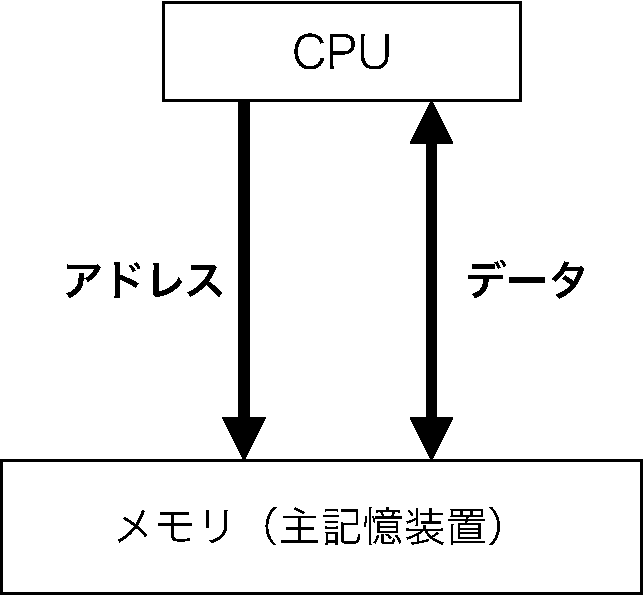
\includegraphics[scale=0.4]{Fig/cpuMemory-crop.pdf}
      \subcaption{単純なモデル}
      \label{fig:cpuMemory}
    \end{center}
  \end{minipage}
  \begin{minipage}{0.49\columnwidth}
    \begin{center}
      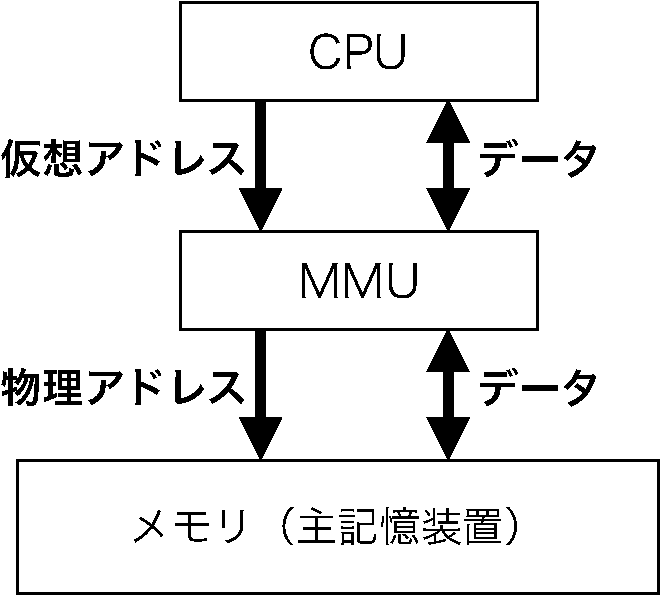
\includegraphics[scale=0.4]{Fig/cpuMmuMemory-crop.pdf}
      \subcaption{仮想化が可能なモデル}
      \label{fig:cpuMmuMemory}
    \end{center}
  \end{minipage}
\end{myfig}

プログラム実行時にCPUは以下のようにメモリをアクセスする.
\begin{enumerate}
\item 命令フェッチ(fetch)\\
  PCの値をアドレスとして出力し主記憶からデータ(命令コード)を\emph{読む}.
\item 命令デコード(decode) \\
  フェッチした命令の種類を調べる.
\item 命令実行(execution)\\
  命令を実行する際に必要に応じてデータのアドレス
  (\emph{実効アドレス:Effective Address(EA)})を出力し
  主記憶のデータを\emph{読み書きする}.
\end{enumerate}

\figref{cpuMemory}のモデルは,
TeCやH8/3664のようなマイクロコンピュータの様子を表すためには十分である.
しかし,この単純なモデルは,
本格的なオペレーティングシステムを作動させるには,次の点で不十分である.
\begin{enumerate}
\item メモリ保護機構がない.\\
  ユーザプロセスがOSのカーネルや,
  他のプロセスを破壊することを防ぐことができない.
\item メモリの再配置機構がない.\\
  同時に複数のプロセスが主記憶にロードされる環境では,
  プロセスの起動と終了が繰り返されるうちに使用できない
  小さなメモリの断片(フラグメント)ができる.
  フラグメントを解消するために,
  実行中プロセスをメモリ内で移動する機能が必要である.
\item 仮想記憶機構が実現できない.\\
  メモリより大きなプログラムを実行するために,
  仮想記憶機構を導入したいができない.
\end{enumerate}

そこで,\figref{cpuMmuMemory}のモデルを用いる.
CPUとメモリの間に
\emph{MMU(Memory Management Unit:メモリ管理装置)}を追加する.
MMUはCPUが出力した\emph{仮想アドレス}をOSが指示したルールに則り
\emph{物理アドレス}に変換してメモリに送るハードウェアである.
\emph{OSの主記憶管理プログラムがMMUを制御することによって,
  使いやすく安全な仮想の主記憶をプロセスに提供する.}

%==============================================================================
\section{メモリ保護機構}
CPUを仮想化したことによって,
複数のユーザプロセスをメモリに同時にロードし並列実行することが可能になった.
これにより,CPUの使用効率が良くなるだけでなく,
コンピュータの使い勝手が非常に良くなった.
しかし,ユーザプログラムのバグや悪意によって,
OSカーネルや他のユーザプログラムが破壊される可能性がでてきた.
OSカーネルはそれの性質上全てのメモリ領域にアクセスする必要がある.
一方でユーザプロセスは自身に割当てられたメモリ以外に
アクセスできない仕組みが必要である.

\subsection{上限・下限レジスタ}
プロセスがアクセスしても良いメモリのアドレスの範囲をレジスタに設定し,
メモリアクセスする度にCPUが出力するアドレスとレジスタの値を比較する.
\figref{baseLimitAddrSpace}はプロセス2が実行中の
上限・下限レジスタの状態を表している.
\figref{baseLimitHardware}はアドレスを比較するハードウェアの
構成を示している.

\begin{myfig}{btp}{上限・下限レジスタの仕組み}{baseLimitRegister}
  \begin{minipage}{0.49\columnwidth}
    \begin{center}
      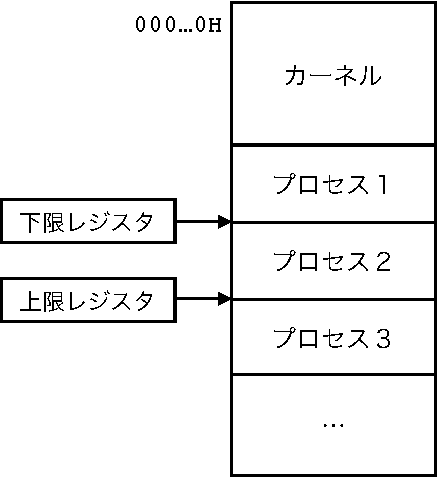
\includegraphics[scale=0.6]{Fig/baseLimitAddrSpace-crop.pdf}
      \subcaption{物理アドレス空間}
      \label{fig:baseLimitAddrSpace}
    \end{center}
  \end{minipage}
  \begin{minipage}{0.49\columnwidth}
    \begin{center}
      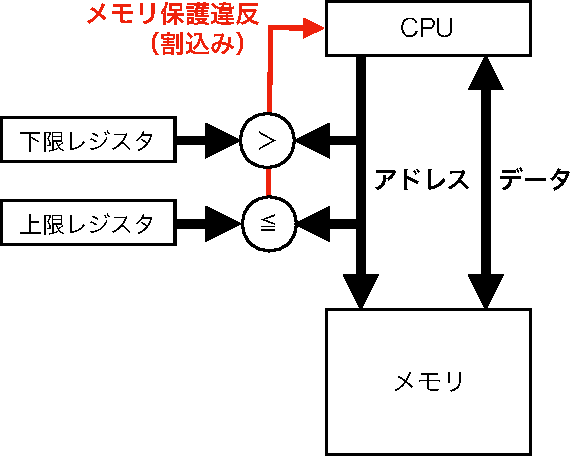
\includegraphics[scale=0.6]{Fig/baseLimitHardware-crop.pdf}
      \subcaption{ハードウェア構成}
      \label{fig:baseLimitHardware}
    \end{center}
  \end{minipage}
\end{myfig}

\begin{enumerate}
\item OSカーネルはプロセスの実行を開始する前に,
  プロセスの上限ドレスと下限ドレスを上限・下限レジスタに設定する.
  上限・下限レジスタを操作できるのはカーネルモード\footnote{
    実行モードは\ref{gen2nd}で紹介したので忘れた人は再確認すること.}で
  実行されるカーネルだけである.
  ユーザプロセスが自身のアクセスできる領域を変更することはできない.
\item カーネルはプロセスの実行を開始させる.
\item プロセスはユーザモードで実行される.
  ユーザモードで実行中は
  ハードウェアがCPUの出力するアドレスを上限・下限レジスタと比較する.
\item 上限・下限アドレスの範囲外へのアクセスの場合,
  ハードウェアがメモリアクセスを阻止しCPUに割込みをかける.
\item 割込みが発生するとユーザプロセスの実行が打ち切られ,
  制御がカーネルに移る.
\end{enumerate}

\subsection{ロック/キー機構}
主記憶をページに分割しページ毎にアクセス許可情報を持たせる.
64KiBのメモリを256ページに分割した例を\figref{lockKeyAddrSpace}に示す.
16bitのアドレスはページ番号を表す上位8bitと,
ページ内オフセットを表す下位8bitに分割される.

\figref{lockKeyHardware}に示すようにCPUは,
アドレス,アクセスキー,R/W/XをMMUに出力する.
アクセスキーはプロセス毎に決まる数字\footnote{プロセス番号でも良い.},
R/W/Xはメモリアクセスの種類を表す次のどれかである.
R(Read)は読み込みを,W(Write)書き込みを,
X(eXecute)は命令のフェッチを意味する.

MMUは許可情報表を内蔵している.
MMUはCPUが出力したアドレスからページ番号を求め表を引く.
表のプロテクションキーがアクセスキーと一致していない場合,
または,CPUのR/W/Xが表のアクセスモードに含まれていない場合は
メモリ保護違反の割込みを発生する.
MMUを操作できるのはCPUの実行モードがカーネルモードの時だけ,
MMUがメモリ保護違反の割込みを発生するのはユーザモード時だけである.

\begin{myfig}{btp}{ロック/キー機構の仕組み}{lockKey}
  \begin{minipage}{0.49\columnwidth}
    \begin{center}
      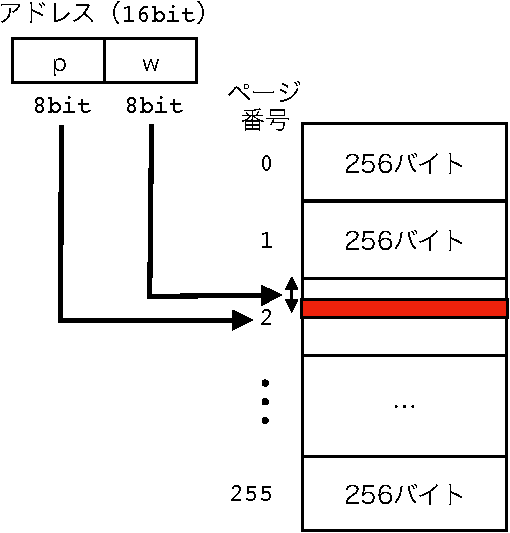
\includegraphics[scale=0.66]{Fig/lockKeyAddrSpace-crop.pdf}
      \subcaption{アドレス空間}
      \label{fig:lockKeyAddrSpace}
    \end{center}
  \end{minipage}
  \begin{minipage}{0.49\columnwidth}
    \begin{center}
      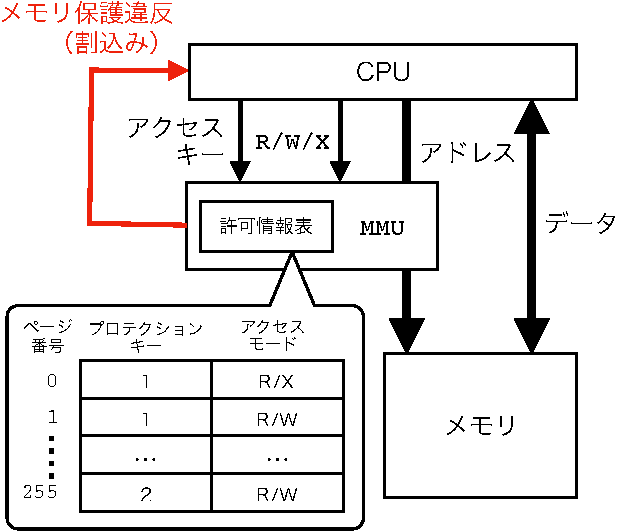
\includegraphics[scale=0.66]{Fig/lockKeyHardware-crop.pdf}
      \subcaption{ハードウェア構成}
      \label{fig:lockKeyHardware}
    \end{center}
  \end{minipage}
\end{myfig}

特別なプロテクションキー(例えば0)のページは
全てのプロセスがアクセス可能とすれば,
プロセス間の共有メモリを実現できる.

%==============================================================================
\section{プログラムの再配置}
コンパイルされたプログラムはメモリにロードされる時にアドレスが確定する.
ファイルに格納された実行可能形式プログラムは,
ロード時にアドレスを変更できる必要がある.

また,実行途中のプログラムのアドレスを変更することがある.
\figref{memoryCompaction}のようにメモリが多くの領域に分断され,
領域の間に小さなメモリの断片(\emph{メモリフラグメント})が沢山できた場合は,
プログラムの詰め合わせ(\emph{メモリコンパクション})を行う.
実行途中のプログラムを移動することを\emph{動的再配置}と呼ぶ.

\begin{myfig}{btp}{プログラムの動的再配置}{memoryCompaction}
  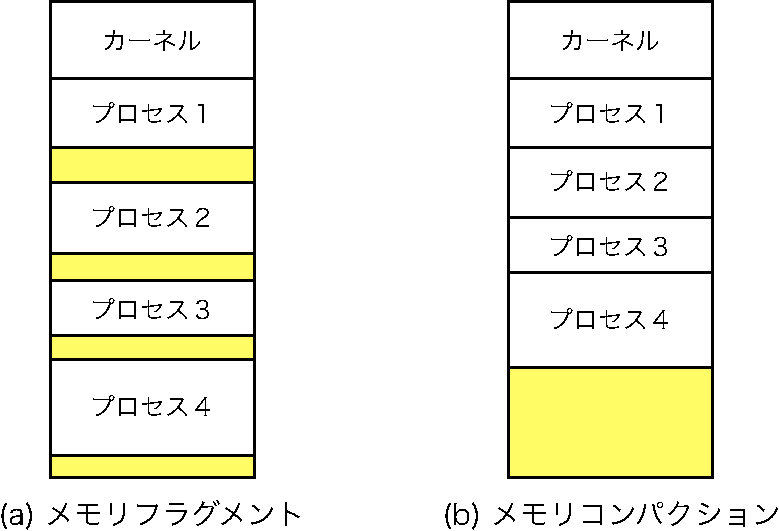
\includegraphics[scale=0.60]{Fig/memoryCompaction-crop.pdf}
\end{myfig}

\subsection{再配置可能オブジェクトファイル}
プログラミング言語で記述されたプログラムは,
コンパイルされ実行可能な機械語ファイルに変換される.
しかしコンパイル時には,
プログラムがメモリの何番地にロードされるか分からない.
そこで,
実行可能形式の機械語プログラムはジャンプ先アドレスや,
データアドレスの確定をロード時に行うことができなければならない.

ロードアドレスが確定しおらず,アドレスを変更可能な機械語プログラムは
\emph{再配置可能オブジェクト(relocatable object)}と呼ばれる.
再配置可能オブジェクトファイルは,
コンパイル済みの機械語プログラムの他に,
プログラム中のどの部分がアドレスであるかを記録した\emph{再配置表}も含む.
プログラムを主記憶にロードする際に再配置表を参照し,
プログラムやデータ中の全てのアドレス情報にロードアドレスを足し込む必要がある.
例えばプログラムを\|1234H|番地にロードすると,
\|JMP 0100H|の機械語は\|JMP 1334H|に書換える必要がある.
ロード時にアドレスを変換する方式を\emph{静的再配置}と呼ぶ.
再配置可能オブジェクトファイルの例としてTacOSが使用する
ファイルのフォーマットを付録\ref{appTacosFileFormat}に示す.

\subsection{リロケーションレジスタ}
動的再配置を行うためには,
実行中のプログラムがどこにアドレスを記憶しているか全て管理する必要がある.
しかし,CPUレジスタやスタックに書き込まれたアドレス,
リスト構造に含まれるポインタ等,
すべてのアドレスデータを追跡することは困難である.

動的再配置を可能にするための一つのアイデアは,
\emph{リロケーションレジスタ}と呼ばれる特別なハードウェアを用いることである.
\figref{relocationAddrSpace}に示すように\footnote{
  図はプロセス2を実行するための設定を表している}
リロケーションレジスタは,
プロセスのロードアドレス(B:Base)と大きさ(L:Limit)を記録するレジスタである.
ディスパッチャがプロセスを実行する時に値を設定する.

\figref{relocationHardware}に示すように
CPUが出力したアドレスはプロセスの大きさ(L)と比較される.
アドレスがL以上の場合はプロセス領域外のアドレスになるので
メモリ保護違反の割込みを発生する.
CPUのアドレスにプロセスのロードアドレス(B)を足した値がメモリアドレスになる.

\begin{myfig}{btp}{リロケーションレジスタ}{relocationRegister}
  \begin{minipage}{0.49\columnwidth}
    \begin{center}
      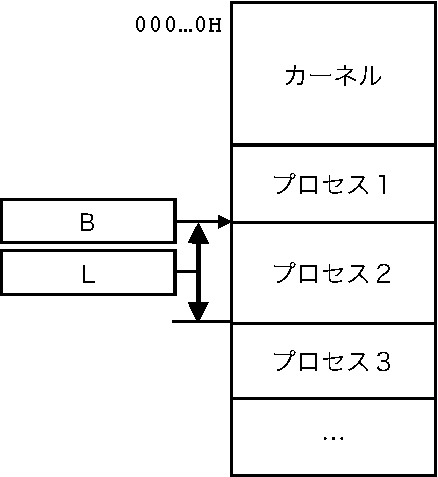
\includegraphics[scale=0.6]{Fig/relocationAddrSpace-crop.pdf}
      \subcaption{物理アドレス空間}
      \label{fig:relocationAddrSpace}
    \end{center}
  \end{minipage}
  \begin{minipage}{0.49\columnwidth}
    \begin{center}
      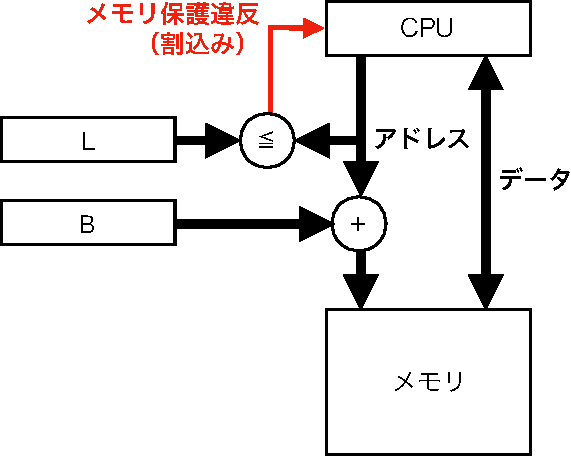
\includegraphics[scale=0.6]{Fig/relocationHardware-crop.pdf}
      \subcaption{ハードウェア構成}
      \label{fig:relocationHardware}
    \end{center}
  \end{minipage}
\end{myfig}

動的再配置を行うにはプロセスがRunning以外の状態の時に,
主記憶上でプロセスのメモリ領域を新しい領域にコピーする.
次回プロセスが実行される時,
ディスパッチャは新しい領域のアドレスをBにロードする.
ユーザプログラムは再配置されたことを知る必要はない.
しかし,プロセスの領域の移動は大量のメモリコピーを伴うので,
\emph{オーバーヘッドが大きい}処理である.

%==============================================================================
\section{アドレス空間の仮想化}
\figref{procOrganization}で示したように,
プロセスは各々が専用の\emph{仮想アドレス空間}(仮想メモリ空間)を持つ.
仮想アドレス空間は仮想アドレスで番地付けされている.
それに対しハードウェアとしてのメモリはシステム全体で一つしかない.
ハードウェアメモリは物理アドレスで番地付けされており,
\emph{物理アドレス空間}を形成する.
\figref{memorySpaceMapping}にプロセスの仮想アドレス空間が,
物理アドレス空間にマッピングされる様子を示す.
マッピングは,MMUよる仮想アドレスから物理アドレスへの変換によってなされる.

\begin{myfig}{btp}{仮想アドレス空間から物理アドレス空間へのマッピング}
  {memorySpaceMapping}
  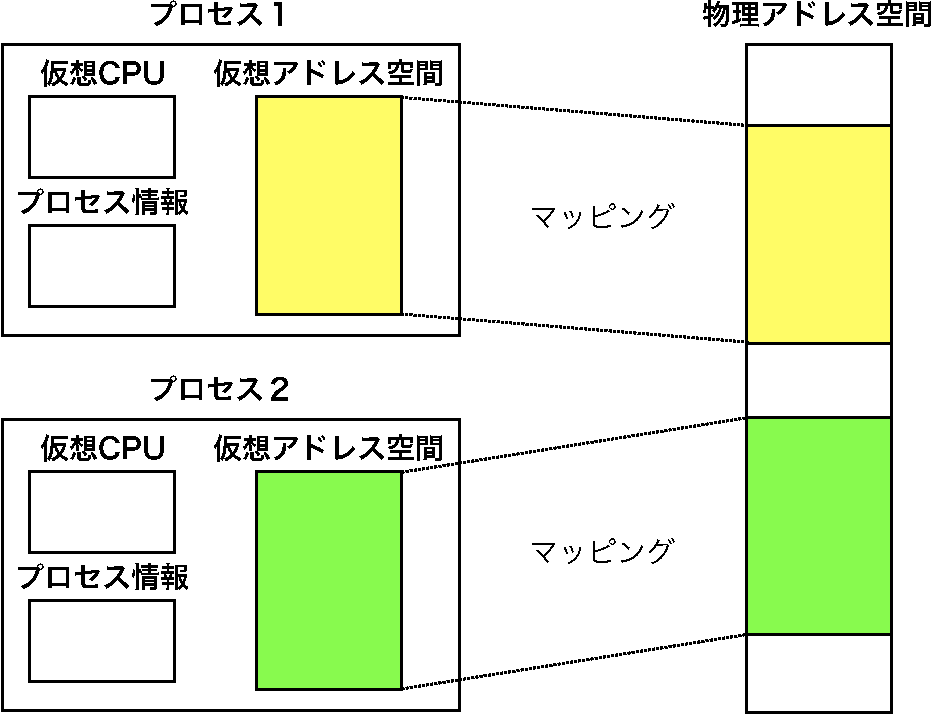
\includegraphics[scale=0.60]{Fig/memorySpaceMapping-crop.pdf}
\end{myfig}

\subsection{単一仮想記憶}
多重仮想記憶に移行する中間的な形式である.
プロセスの仮想アドレスと物理アドレスが同じ方式である.
メリットが少ないので通常は次に紹介する多重仮想記憶を用いる.

\subsection{多重仮想記憶}
アドレス空間が仮想化されることにより,
全てのプロセスが0番地から始まるアドレス空間を持つことが可能になる.
プロセス毎に独立したアドレス空間を持つ方式を\emph{多重仮想記憶}と呼ぶ.
実行可能形式のプログラムは,いつも0番地にロードされ実行される.
%再配置可能なオブジェクトでなくても良い.

\subsection{仮想アドレス空間の配置}
仮想アドレス空間にプログラムや変数を配置する方法は
オペレーティングシステムの種類により一定ではない.
\figref{memoryMapVsClang}とリスト\ref{cmmSample}に
UNIX上でC言語プログラムが配置される様子を示す.

\begin{myfig}{btp}{仮想アドレス空間の配置例}{memoryMapVsClang}
  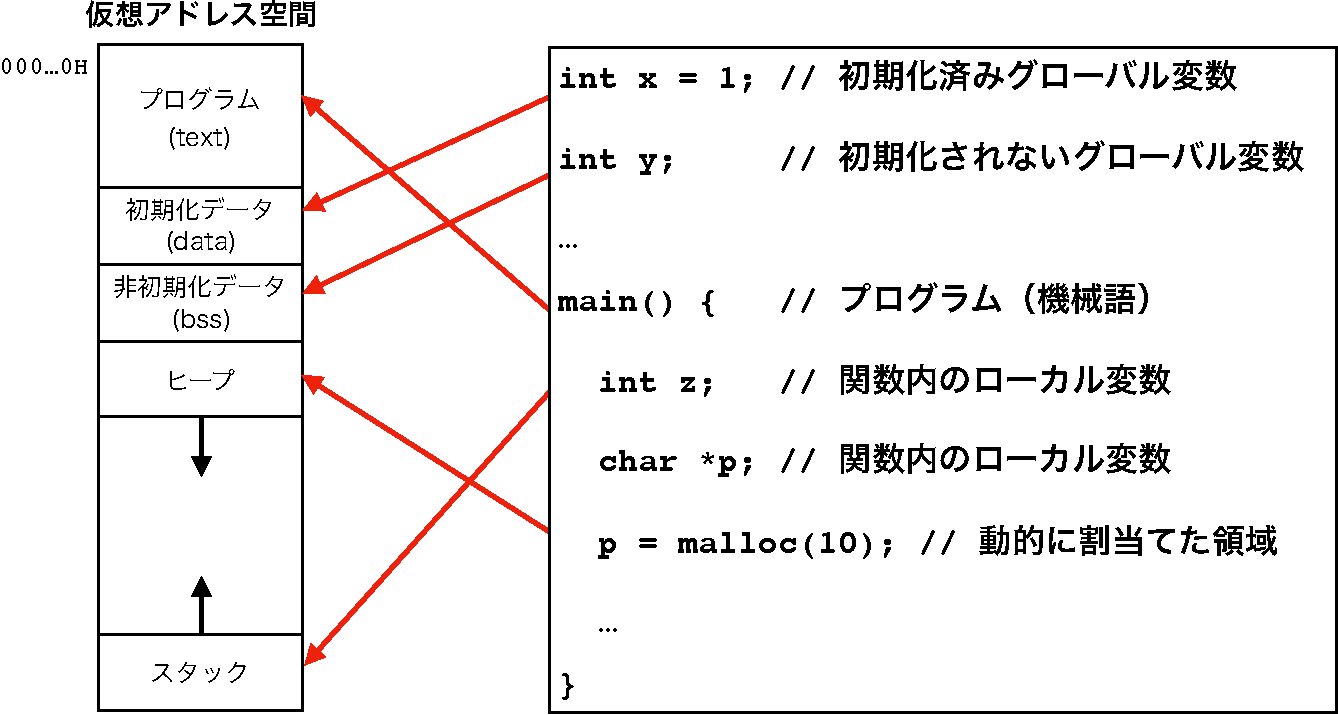
\includegraphics[scale=0.6]{Fig/memoryMapVsClang-crop.pdf}
\end{myfig}

\begin{itemize}
\item 初期化済みのグローバル変数\footnote{
  正確には初期化済みの静的な変数.
  関数内で\texttt{static}修飾した変数も含まれる.}は,
  初期化データ領域(\emph{dataセグメント})に配置される.
\item 初期化されないグローバル変数\footnote{
  正確には初期化されない静的な変数.
  関数内で\texttt{static}修飾した変数も含まれる.}は,
  非初期化データ領域(\emph{bssセグメント})に配置される.
\item \texttt{main()}関数は機械語に変換され,
  プログラム領域(\emph{textセグメント})に配置される.
\item 関数のローカル変数\footnote{
  正確には自動変数.
  関数内で\texttt{static}修飾した変数は含まれない.}は,
  関数の実行開始時に\emph{スタックセグメント}または
  \emph{CPUレジスタ}に割り付けられ,
  関数を終了する時に破棄される.
  同じスタックを関数呼出しのために CALL 機械語命令も使用する.
  スタックは,必要に応じて仮想アドレス空間を0番地側に伸びる.
\item \|malloc()|関数等を用いて動的に領域を割り当てると
  \emph{ヒープセグメント}が使用される.
  ヒープは必要に応じて仮想アドレス空間を0番地とは逆の方向に伸びる.
\end{itemize}

\lstinputlisting[caption=C言語プログラムをTaCの機械語に変換した例,
  numbers=none,float=btp,label=cmmSample]{Lst/cmmSample.s}

%==============================================================================
\section{まとめ}
主記憶(メモリ)は,
プログラムや変数をロードし,
CPUがプログラムを実行する際に直接使用する記憶装置である.
メモリ保護機構には\emph{上限・下限レジスタ},\emph{ロック/キー機構}があった.
プログラムの再配置は,
プログラムをメモリにロードする時点で行う\emph{静的再配置}と,
プログラム実行中に行う\emph{動的再配置}があった.
静的再配置は\emph{再配置可能オブジェクトファイル}に格納された
\emph{再配置表}を用いて行う.
動的再配置には,ハードウェアの支援が必要である.
このようなハードウェアの例は\emph{リロケーションレジスタ}である.

メモリ保護やプログラムの動的再配置を行うために,
MMUと呼ばれるハードウェアをCPUとメモリの間に配置する.
MMUは\emph{仮想アドレス}を\emph{物理アドレス}に
マッピングするアドレス変換器として働く.
マッピング方法をプロセス毎に変更することで\emph{多重仮想記憶}が実現できる.
仮想アドレス空間の配置をUNIXを例に紹介した.
UNIXプロセスの仮想アドレス空間は,
text,data,bss,ヒープ,スタックセグメントからなる.

%==============================================================================
\section*{練習問題}
\begin{enumerate}
  \renewcommand{\labelenumi}{\ttfamily\arabic{chapter}.\arabic{enumi}}
  \setlength{\leftskip}{1em}
\item 次の言葉の意味を説明しなさい.
  \begin{enumerate}
  \item 主記憶(メモリ)
  \item MMU
  \item メモリ保護
  \item 上限・下限レジスタ
  \item 静的再配置
  \item 動的再配置
  \item 再配置可能オブジェクトファイル
  \item リロケーションレジスタ
  \item 仮想アドレス空間
  \item 物理アドレス空間
  \item 多重仮想記憶
  \item textセグメント
  \item dataセグメント
  \item bssセグメント
  \item ヒープセグメント
  \item スタックセグメント
  \end{enumerate}
\item 自分がいつも使用しているPCの主記憶(メモリ)は何GBか調べなさい.
\item 上限・下限レジスタは,プログラムの動的再配置のために使用できるか?
\item 付録\ref{appTacosFileFormat}に示すTacOSのファイルフォーマットの中で,
  再配置可能オブジェクトファイルの構造を理解しなさい.
\item リスト\ref{cmmSample}のプログラムの場合,
  リロケーションレコードはいくつ必要か?
\end{enumerate}
